%%%%%%%%%%%%%%%%%%%%%%%%%%%%%%%%%%%%%%%%%
% Short Sectioned Assignment
% LaTeX Template
% Version 1.0 (5/5/12)
%
% This template has been downloaded from:
% http://www.LaTeXTemplates.com
%
% Original author:
% Frits Wenneker (http://www.howtotex.com)
%
% License:
% CC BY-NC-SA 3.0 (http://creativecommons.org/licenses/by-nc-sa/3.0/)
%
%%%%%%%%%%%%%%%%%%%%%%%%%%%%%%%%%%%%%%%%%

%----------------------------------------------------------------------------------------
%	PACKAGES AND OTHER DOCUMENT CONFIGURATIONS
%----------------------------------------------------------------------------------------

\documentclass[titlepage, paper=a4, fontsize=11pt]{scrartcl} % A4 paper and 11pt font size

\usepackage[T1]{fontenc} % Use 8-bit encoding that has 256 glyphs
\usepackage{fourier} % Use the Adobe Utopia font for the document - comment this line to return to the LaTeX default
\usepackage[english]{babel} % English language/hyphenation
\usepackage{amsmath,amsfonts,amsthm} % Math packages
\usepackage{listings}

\usepackage{lipsum} % Used for inserting dummy 'Lorem ipsum' text into the template
\usepackage{graphicx}
\usepackage{caption}


\usepackage{sectsty} % Allows customizing section commands
\allsectionsfont{\centering \normalfont\scshape} % Make all sections centered, the default font and small caps

\usepackage{fancyhdr} % Custom headers and footers
\pagestyle{fancyplain} % Makes all pages in the document conform to the custom headers and footers
\fancyhead{} % No page header - if you want one, create it in the same way as the footers below
\fancyfoot[L]{} % Empty left footer
\fancyfoot[C]{} % Empty center footer
\fancyfoot[R]{\thepage} % Page numbering for right footer
\renewcommand{\headrulewidth}{0pt} % Remove header underlines
\renewcommand{\footrulewidth}{0pt} % Remove footer underlines
\setlength{\headheight}{13.6pt} % Customize the height of the header

\numberwithin{equation}{section} % Number equations within sections (i.e. 1.1, 1.2, 2.1, 2.2 instead of 1, 2, 3, 4)
\numberwithin{figure}{section} % Number figures within sections (i.e. 1.1, 1.2, 2.1, 2.2 instead of 1, 2, 3, 4)
\numberwithin{table}{section} % Number tables within sections (i.e. 1.1, 1.2, 2.1, 2.2 instead of 1, 2, 3, 4)

\setlength\parindent{0pt} % Removes all indentation from paragraphs - comment this line for an assignment with lots of text

%----------------------------------------------------------------------------------------
%	TITLE SECTION
%----------------------------------------------------------------------------------------

\newcommand{\horrule}[1]{\rule{\linewidth}{#1}} % Create horizontal rule command with 1 argument of height

\title{	
\normalfont \normalsize 
\textsc{University of Virginia} \\ [25pt] % Your university, school and/or department name(s)
\horrule{0.5pt} \\[0.4cm] % Thin top horizontal rule
\huge ECE/CS 5565 Project 1 \\ % The assignment title
\horrule{2pt} \\[0.5cm] % Thick bottom horizontal rule
}

\renewcommand{\thefigure}{\arabic{figure}}

\author{Shawn (Shuoshuo) Chen\\sc7cq@virginia.edu} % Your name

\date{\normalsize\today} % Today's date or a custom date

\begin{document}

\maketitle % Print the title

%----------------------------------------------------------------------------------------
%	PROBLEM 1
%----------------------------------------------------------------------------------------

\section*{\textbf{Lab 1}}
\subsection*{Question 1}
DHCP, DNS, ARP
\\

\subsection*{Question 2}
HTTP GET was sent at 22:34:56.094124999 and the HTTP OK was received at 22:34:56.115811000.
It took about 0.02 seconds (20 milliseconds).
\\

\subsection*{Question 3}
The Internet address of gaia.cs.umass.edu is $128.119.245.12$. The Internet address of my
computer is $128.143.137.117$.
\\

\subsection*{Question 4}
See Figure ~\ref{fig:http}.
\\[12pt]


\section*{\textbf{Lab 2}}
\begin{figure}[!ht]
    \centering
    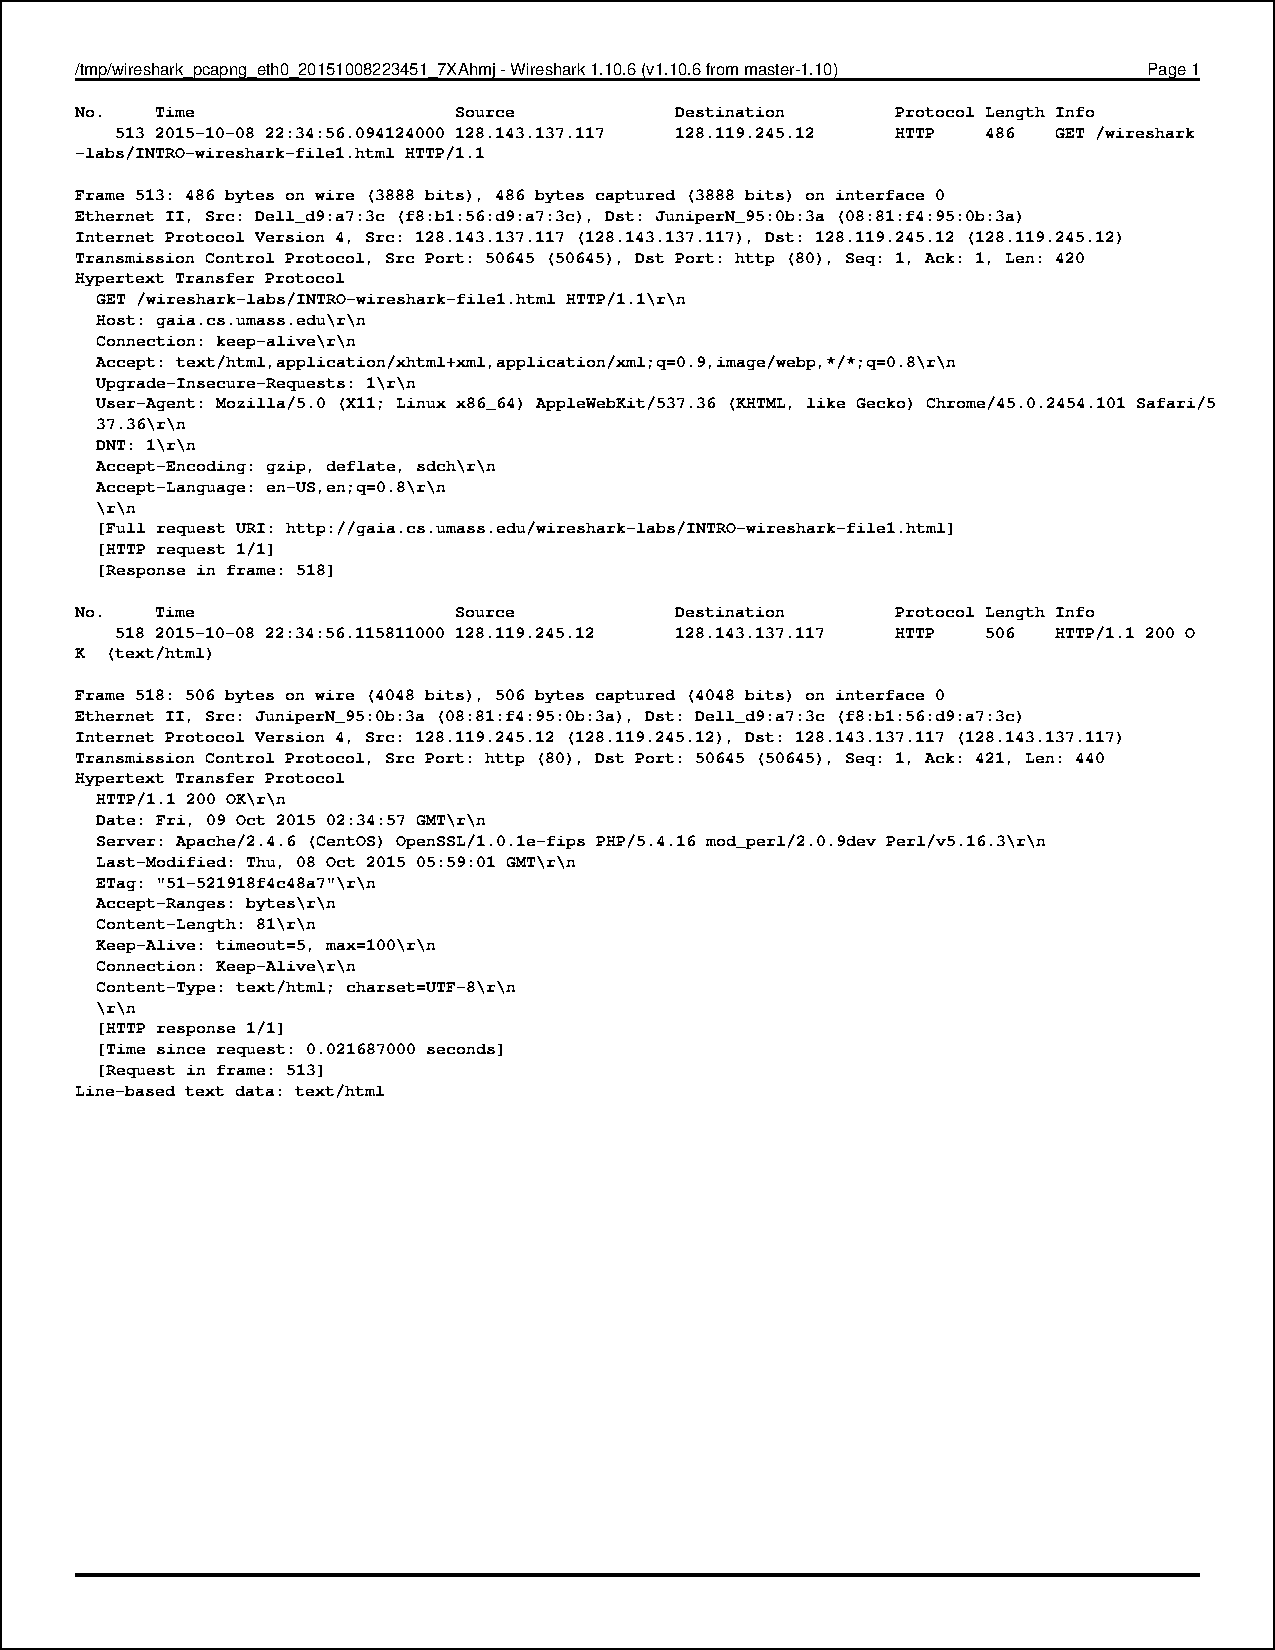
\includegraphics[width=\textwidth]{images/http-cap.pdf}
    \caption{HTTP GET and response}
    \label{fig:http}
\end{figure}

\subsection*{Question 1}
My browser is running HTTP 1.1. It can be found from the GET packet:
\begin{verbatim}
GET /wireshark-labs/HTTP-wireshark-file1.html HTTP/1.1\r\n
\end{verbatim}

The server is running HTTP 1.1. It can be found from the response packet:
\begin{verbatim}
HTTP/1.1 200 OK\r\n
\end{verbatim}


\subsection*{Question 2}
English. It can be found from the GET packet:
\begin{verbatim}
Accept-Language: en-US,en;q=0.8\r\n
\end{verbatim}


\subsection*{Question 3}
IP of my computer is 128.143.137.117, IP of gaia.cs.umass.edu is 128.119.245.12.
This can be found from the IP header of the GET packet.
\begin{verbatim}
Internet Protocol Version 4, Src: 128.143.137.117 (128.143.137.117),
Dst: 128.119.245.12 (128.119.245.12)
\end{verbatim}


\subsection*{Question 4}
Status code is 200. This is found from the response packet:
\begin{verbatim}
HTTP/1.1 200 OK\r\n
\end{verbatim}


\subsection*{Question 5}
It was last modified at 05:59:01 GMT on Oct. 8th, 2015. This is found from the response packet:
\begin{verbatim}
Last-Modified: Thu, 08 Oct 2015 05:59:01 GMT\r\n
\end{verbatim}


\subsection*{Question 6}
The content length is 128 bytes, found from the response packet:
\begin{verbatim}
Content-Length: 128\r\n
\end{verbatim}


\subsection*{Question 7}
Yes. Within the response body, there is a `Line-based text data: text/html' filed.
If expand the field, we will see the source code of that page inside:
\begin{verbatim}
<html>\n
Congratulations.  You've downloaded the file \n
http://gaia.cs.umass.edu/wireshark-labs/HTTP-wireshark-file1.html!\n
</html>\n
\end{verbatim}


\begin{figure}[!ht]
    \centering
    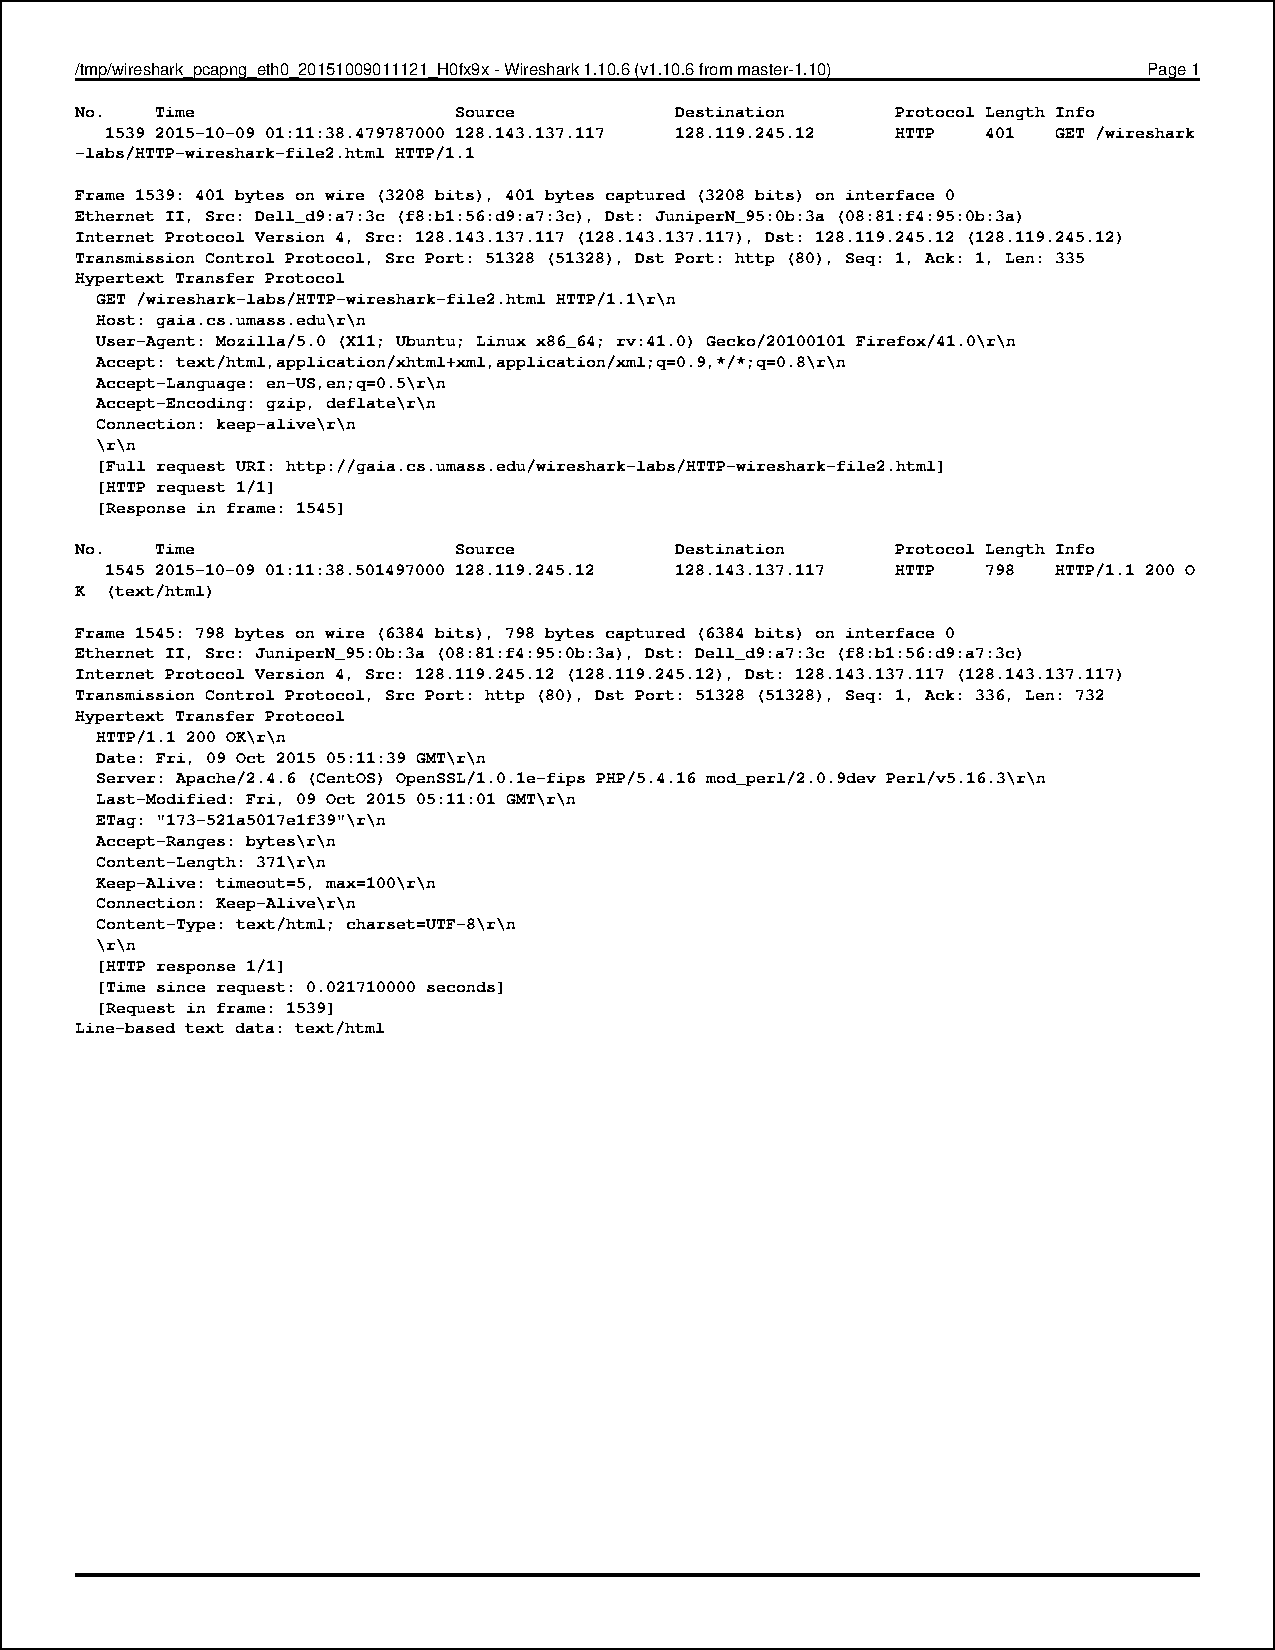
\includegraphics[width=\textwidth]{images/cond-get1.pdf}
    \caption{HTTP Conditional GET with no cache}
    \label{fig:cond-get1}
\end{figure}
\begin{figure}[!ht]
    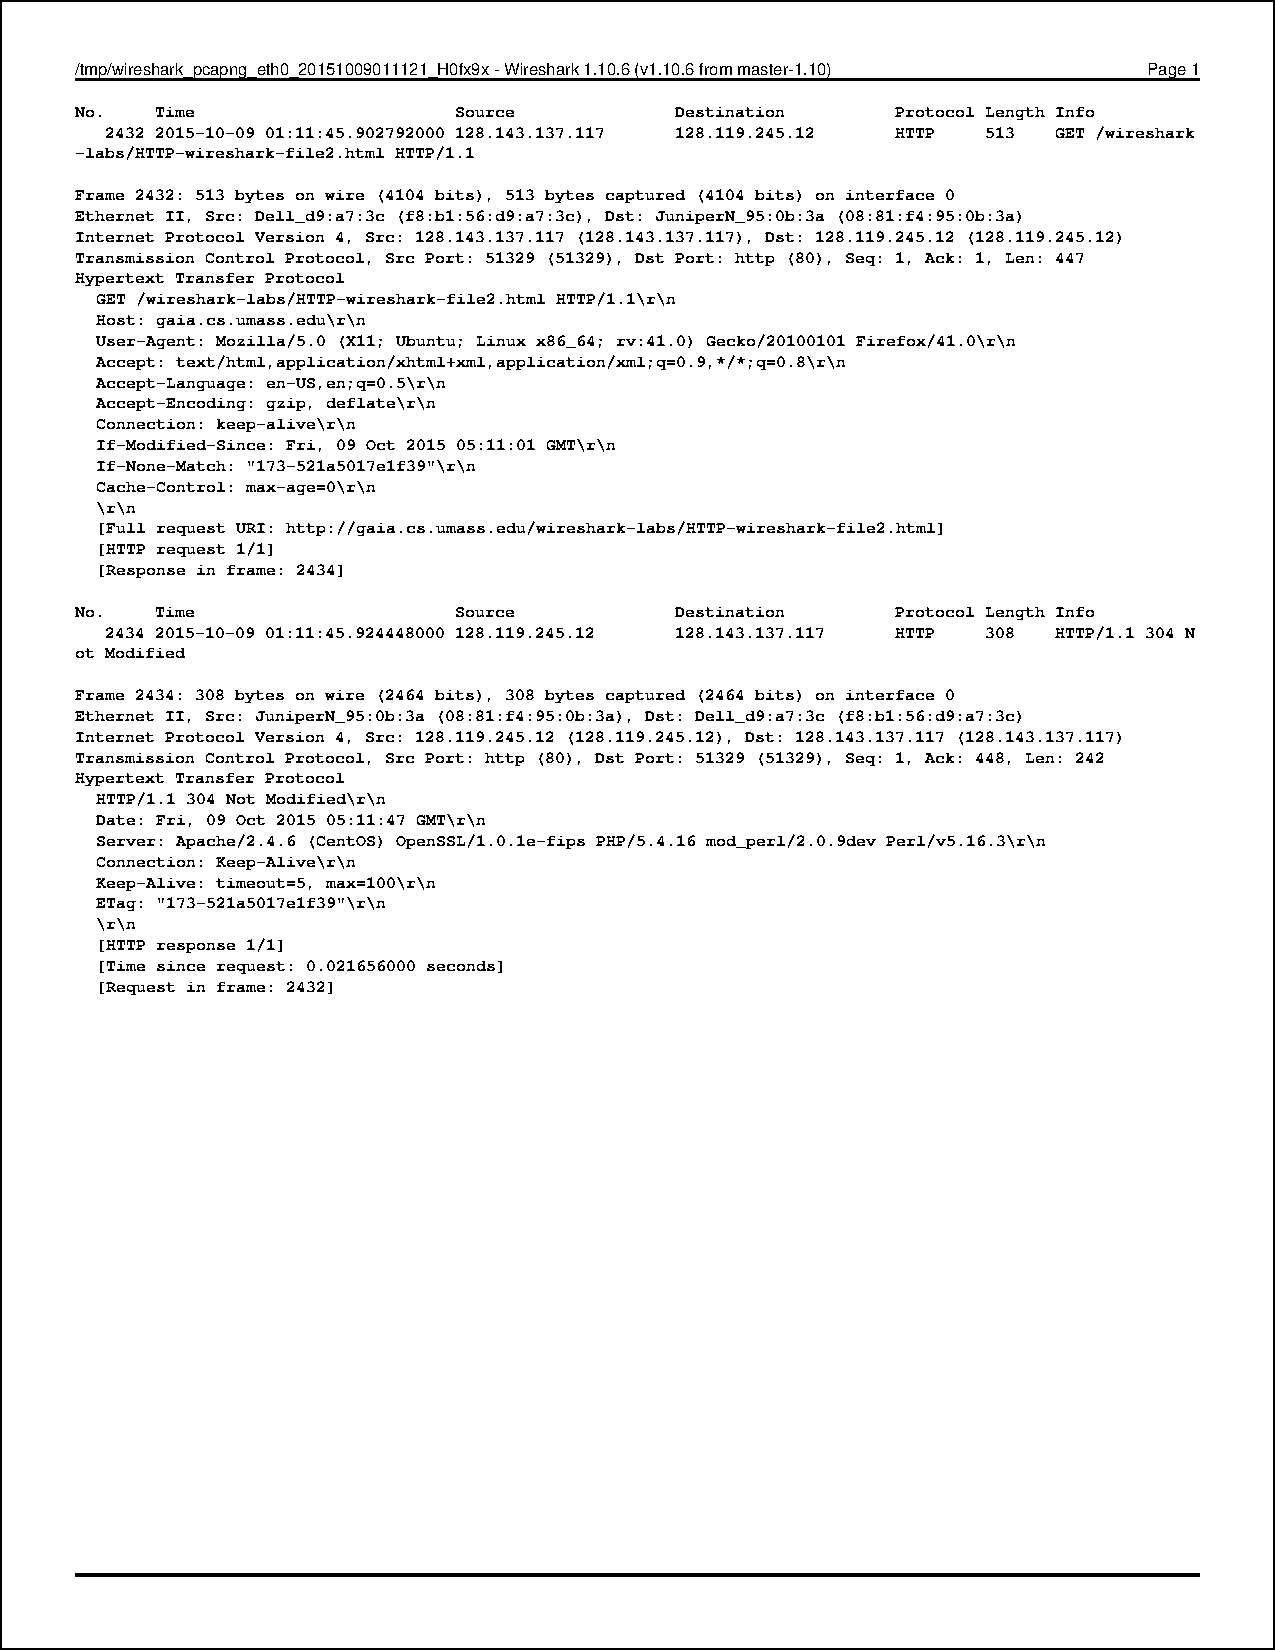
\includegraphics[width=\textwidth]{images/cond-get2.pdf}
    \caption{HTTP Conditional GET with cache}
    \label{fig:cond-get2}
\end{figure}

\newpage
%\noindent\makebox[\linewidth]{\rule{\textwidth}{0.4pt}}
%\\[12pt]
The two pairs of HTTP GET and response packets are displayed in Figure ~\ref{fig:cond-get1}
and Figure ~\ref{fig:cond-get2}.

\subsection*{Question 8}
No, I do not see.
\\


\subsection*{Question 9}
Yes, by expanding the field `Line-based text data: text/html', I can see the source code of
the requested page. As following shows:
\begin{verbatim}
Line-based text data: text/html
\n
<html>\n
\n
Congratulations again!  Now you've downloaded the file lab2-2.html.
<br>\n
This file's last modification date will not change.  <p>\n
Thus  if you download this multiple times on your browser, a
complete copy <br>\n
will only be sent once by the server due to the inclusion of the
IN-MODIFIED-SINCE<br>\n
field in your browser's HTTP GET request to the server.\n
\n
</html>\n
\end{verbatim}


\subsection*{Question 10}
Yes, the followed information is: Fri, 09 Oct 2015 05:11:01 GMT.
And the field from the packet:
\begin{verbatim}
If-Modified-Since: Fri, 09 Oct 2015 05:11:01 GMT\r\n
\end{verbatim}


\subsection*{Question 11}
The returned status code is 304 Not Modified.
\begin{verbatim}
HTTP/1.1 304 Not Modified\r\n
Fri, 09 Oct 2015 05:11:47 GMT
\end{verbatim}
No, the server did not return the content because the server checked the
If-Modified-Since field in the request and found that the requested object
has not been modified. According to the note that the server updates the
modified time of that object every minute, we can see that the second request
was sent within one minute. Thus the server just returned 304 instead the object.

\newpage


\begin{figure}[!ht]
    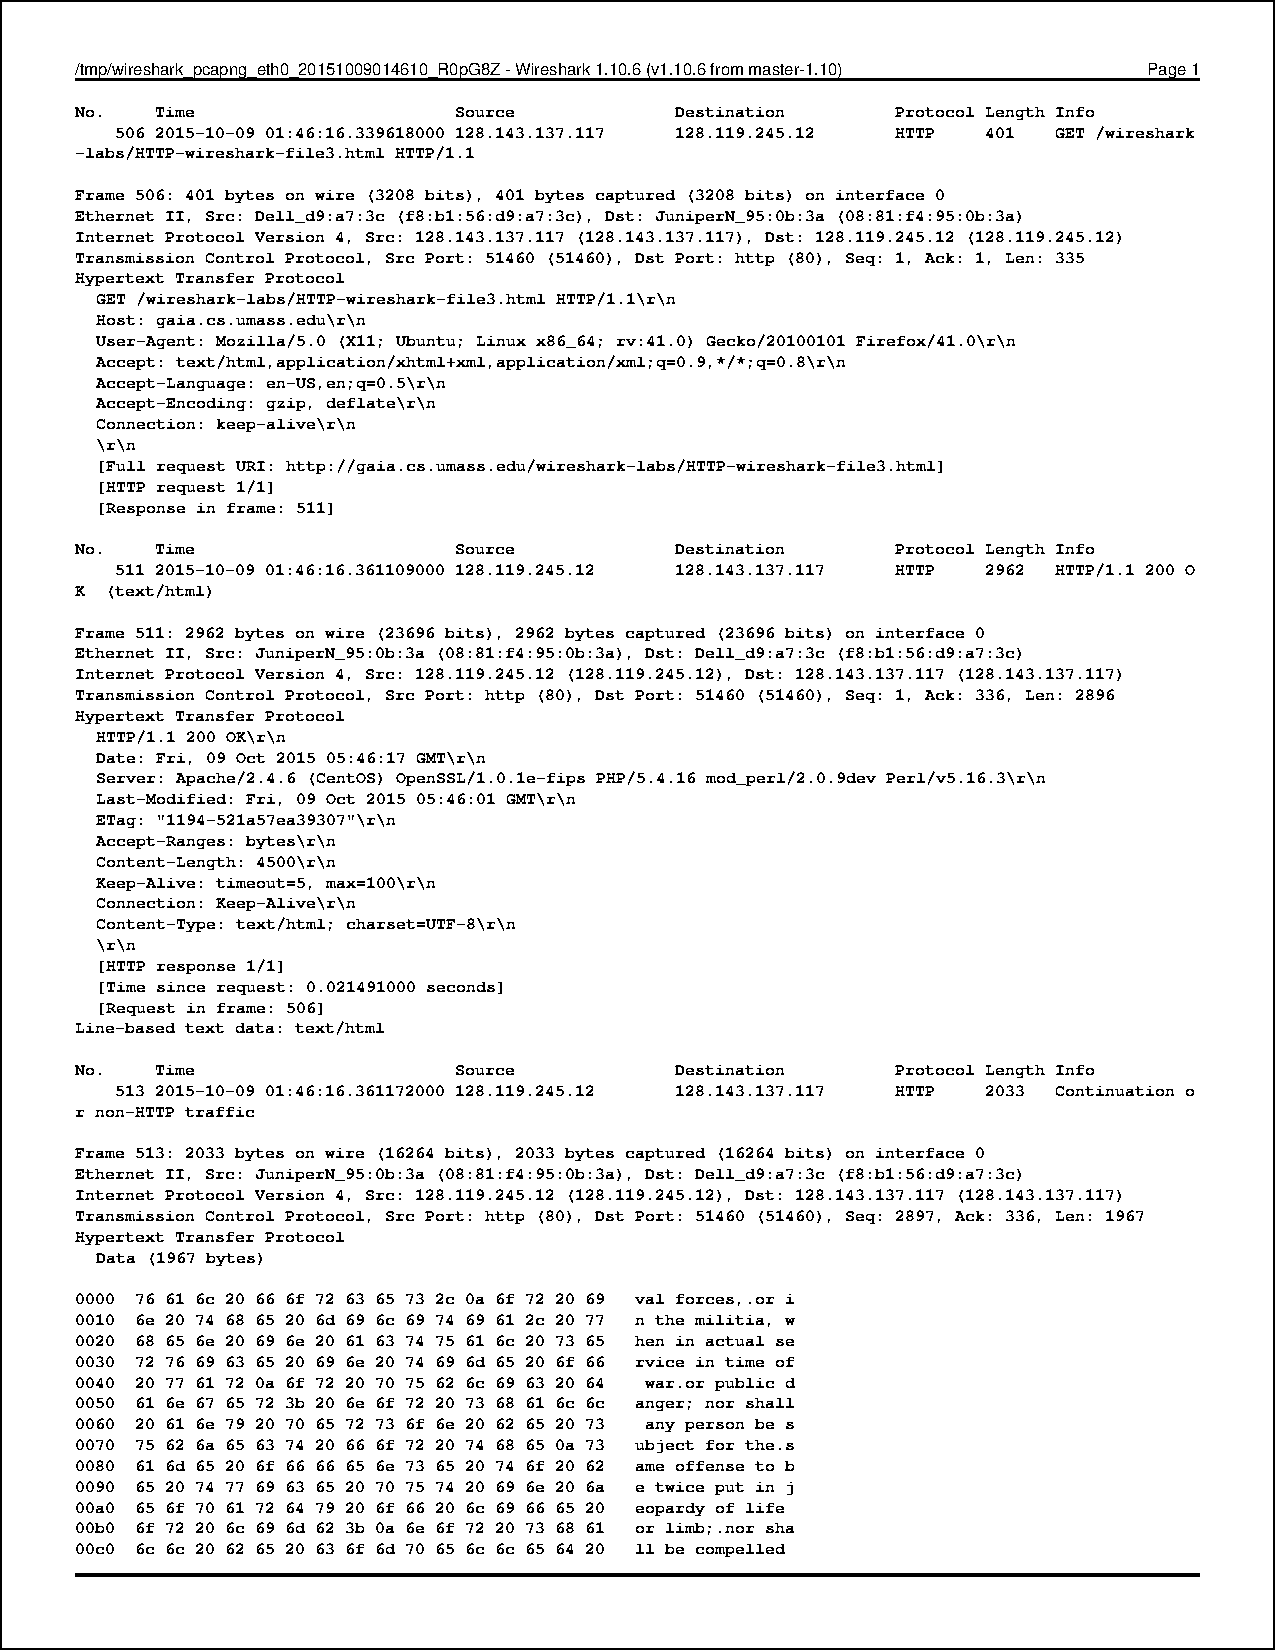
\includegraphics[width=\textwidth]{images/longobj.pdf}
    \caption{HTTP Long Document}
    \label{fig:longobj}
\end{figure}

The HTTP GET and response for US Bill of Rights are displayed in Figure ~\ref{fig:longobj}.
\\

\subsection*{Question 12}
Just one. The packet number is 506.
\\


\subsection*{Question 13}
Packet 511 contains the status code and phrase as showed:
\begin{verbatim}
No  Time        Source         Destination     Protocol Length
511	5.539201000	128.119.245.12 128.143.137.117 HTTP     2962
...
HTTP/1.1 200 OK\r\n
\end{verbatim}


\subsection*{Question 14}
The status code is 200 and phrase is OK same as showed in question 13.
\\


\subsection*{Question 15}
Two segments were needed. First one came with a response of status code and
a part of the text, which the TCP payload (HTTP content) is 2896 bytes.
Second one came with the rest of the text, which the payload is 1967 bytes.
This can be seen in Figure ~\ref{fig:longobj}.

\newpage


\begin{figure}[!ht]
    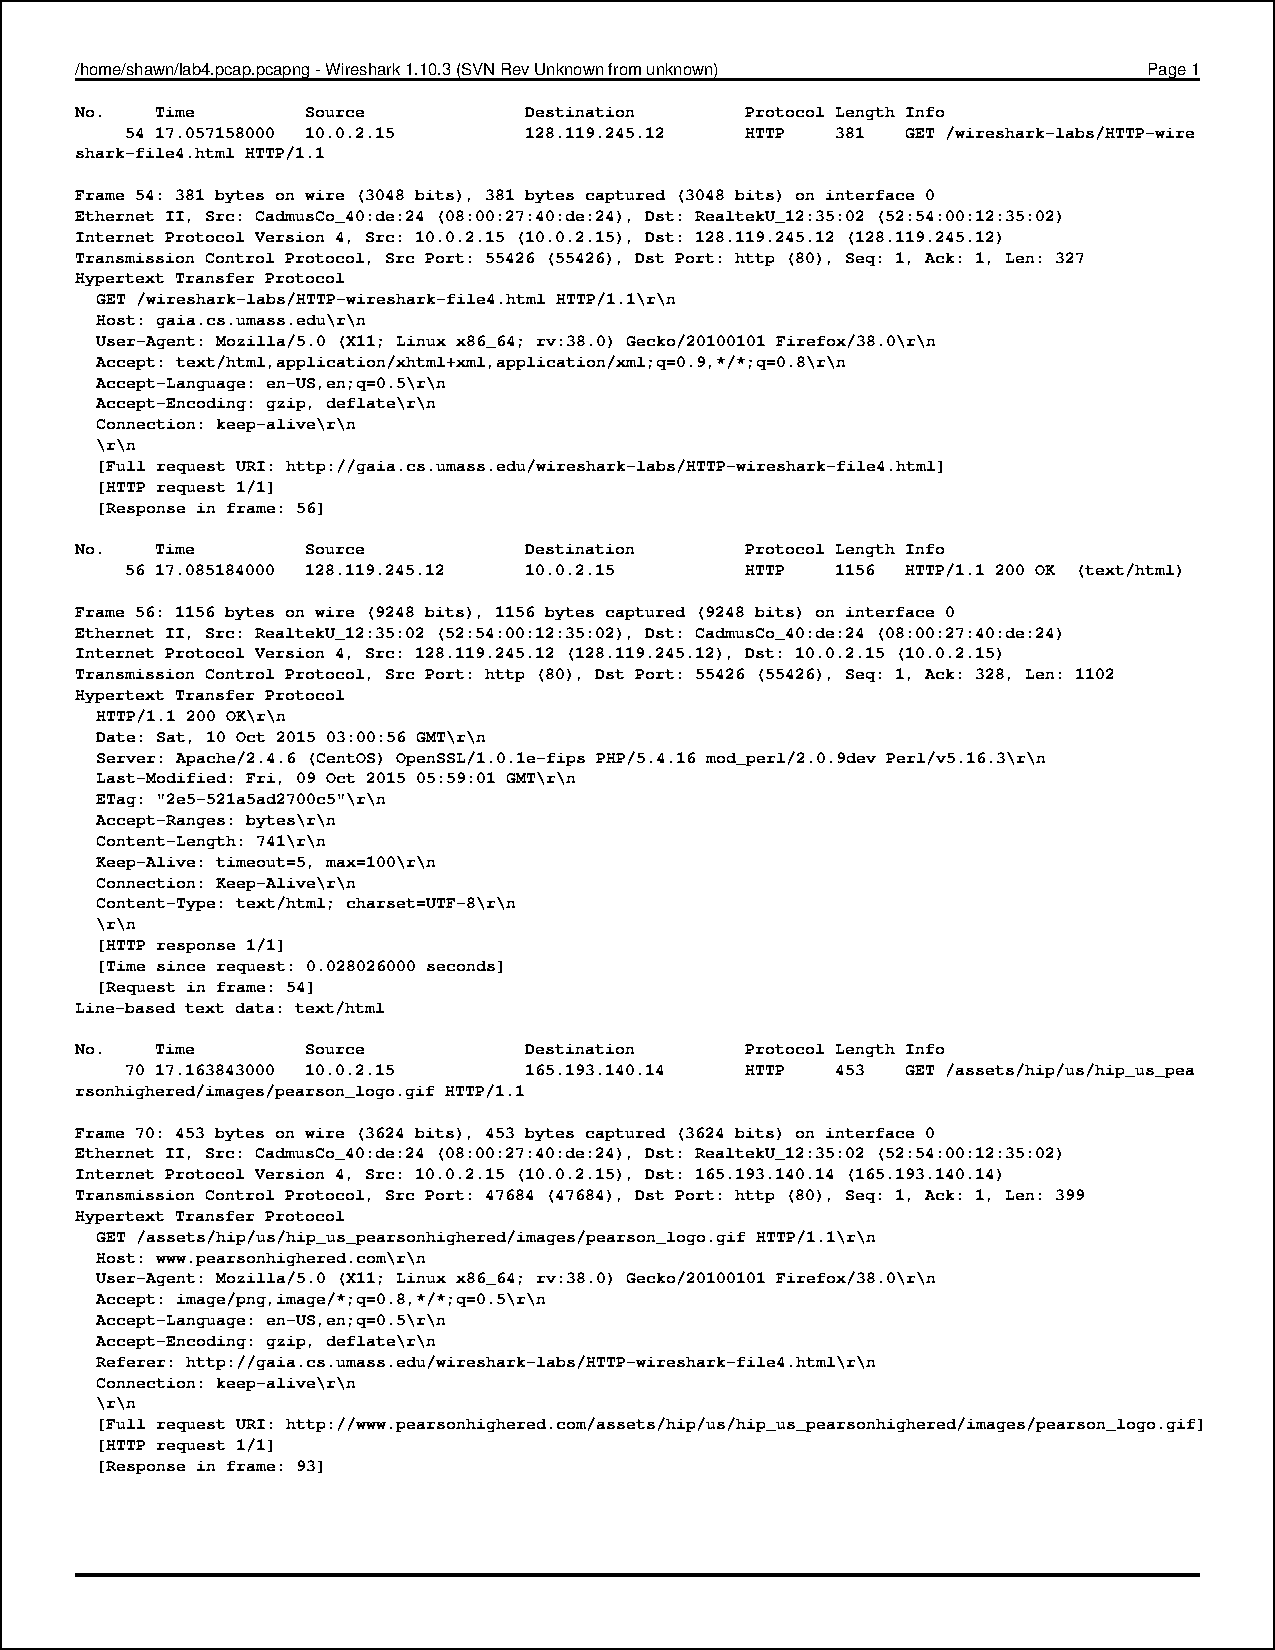
\includegraphics[width=\textwidth]{images/refobj1.pdf}
    \caption{HTTP Document with Embedded Objects 1}
    \label{fig:refobj1}
\end{figure}
\begin{figure}[!ht]
    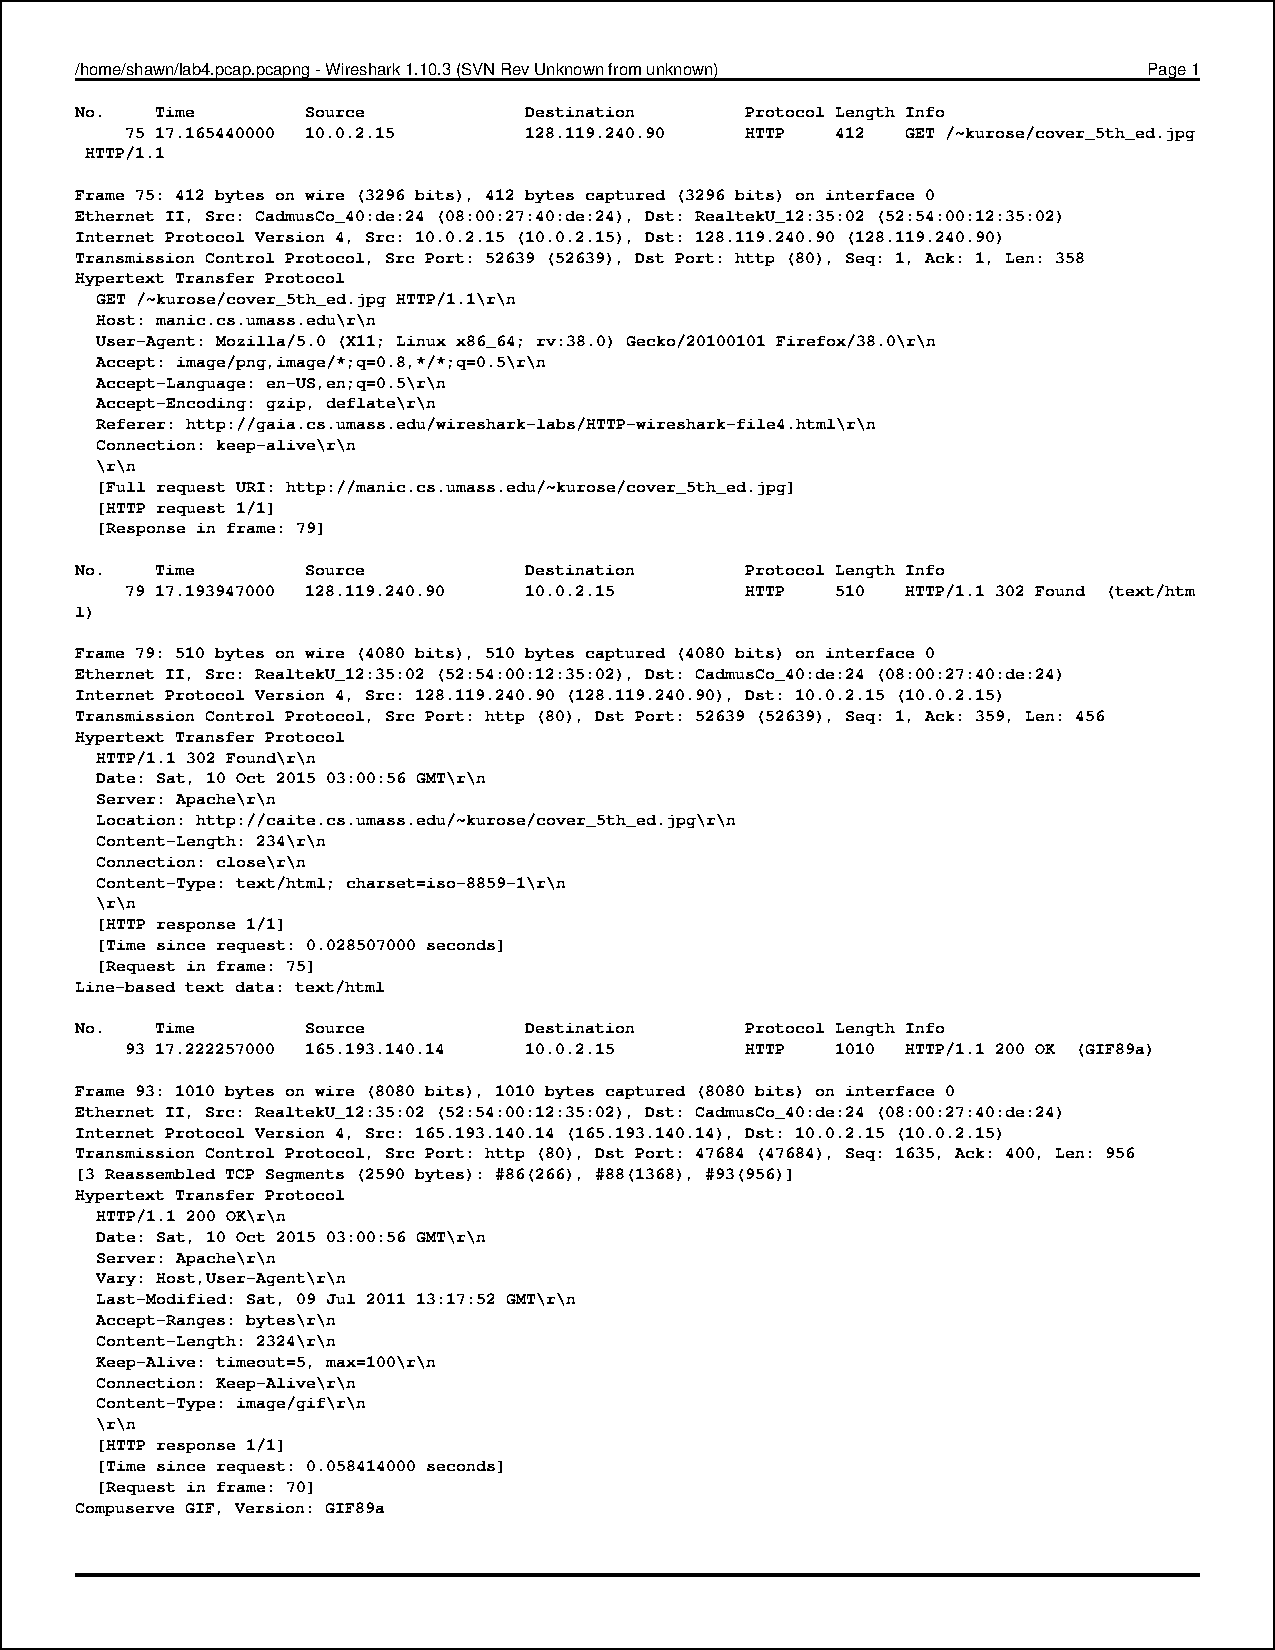
\includegraphics[width=\textwidth]{images/refobj2.pdf}
    \caption{HTTP Document with Embedded Objects 2}
    \label{fig:refobj2}
\end{figure}
\begin{figure}[!ht]
    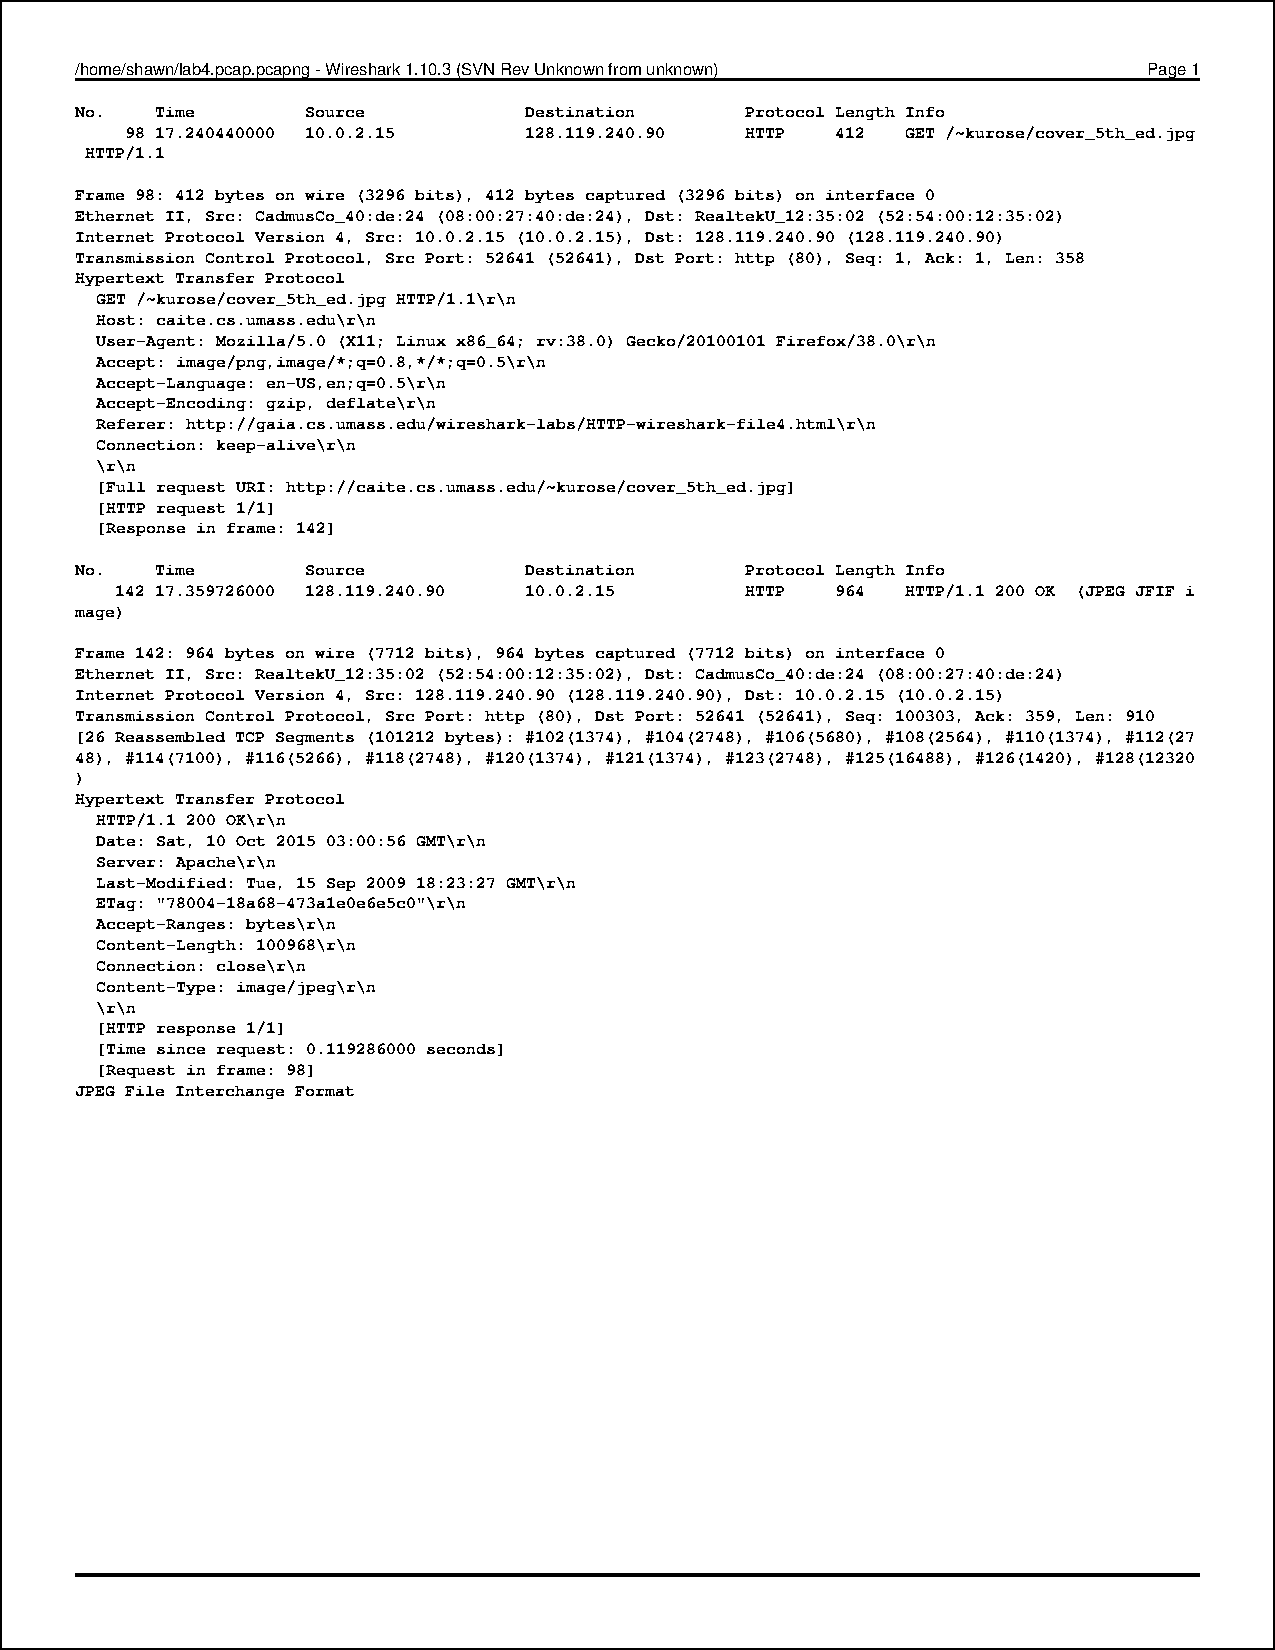
\includegraphics[width=\textwidth]{images/refobj3.pdf}
    \caption{HTTP Document with Embedded Objects 3}
    \label{fig:refobj3}
\end{figure}

\newpage
The HTTP document with embedded objects are displayed in Figure ~\ref{fig:refobj1}, Figure ~\ref{fig:refobj2} and Figure ~\ref{fig:refobj3}.
\\

\subsection*{Question 16}
My browser sent 4 HTTP GET messages. \\
The first GET was sent to 128.119.245.12
(gaia.cs.umass.edu) to retrieve the base page:
\begin{verbatim}
No  Time        Source      Destination       Protocol  Length    Info
54  17.057158   10.0.2.15	  128.119.245.12    HTTP      381       GET
/wireshark-labs/HTTP-wireshark-file4.html HTTP/1.1
\end{verbatim}
The second GET was sent to 165.193.140.14 (www.pearsonhighered.com) to retrieve the logo:
\begin{verbatim}
No  Time        Source      Destination       Protocol  Length    Info
70  17.163843   10.0.2.15   165.193.140.14	   HTTP      453       GET
/assets/hip/us/hip_us_pearsonhighered/images/pearson_logo.gif HTTP/1.1 
\end{verbatim}
The third GET was sent to 128.119.240.90 (manic.cs.virginia.edu) to retrieve the cover page:
\begin{verbatim}
No  Time        Source      Destination       Protocol  Length    Info
75  17.165440   10.0.2.15   128.119.240.90    HTTP      412       GET
/~kurose/cover_5th_ed.jpg HTTP/1.1 
\end{verbatim}
The fourth GET was sent to 128.119.240.90 (caite.cs.umass.edu) because manic.cs.virginia.edu told the browser that the cover page is moved to another place:
\begin{verbatim}
No  Time        Source      Destination       Protocol  Length    Info
98  17.240440   10.0.2.15   128.119.240.90    HTTP      412       GET
/~kurose/cover_5th_ed.jpg HTTP/1.1 
\end{verbatim}

\subsection*{Question 17}
The two images were downloaded in parallel. Wireshark shows there were two GET messages going out almost at the same time (one for logo and the other for cover page). Then two responses came in.
\begin{verbatim}
No  Time        Source      Destination       Protocol  Length    Info
70  17.163843   10.0.2.15   165.193.140.14	   HTTP      453       GET
/assets/hip/us/hip_us_pearsonhighered/images/pearson_logo.gif HTTP/1.1
75  17.165440   10.0.2.15   128.119.240.90    HTTP      412       GET
/~kurose/cover_5th_ed.jpg HTTP/1.1
79  17.193947   128.119.240.90  10.0.2.15     HTTP      510       HTTP/1.1
302 Found
93  17.222257   165.193.140.14  10.0.2.15     HTTP      1010      HTTP/1.1
200 OK  (GIF89a)
\end{verbatim}
Note the request pattern is GET-GET-Response-Response, which means it is parallel. A serial pattern should look like GET-Response-GET-Response. \\

The two GET messages were going out with a minor gap because the browser parses the base page in sequence.
Once the browser finds a referenced object, it issues a request immediately. Since the logo is referenced in the base page prior to the cover page, there is difference in time. \\

Also, even the cover page was not successfully retrieved in the first response, the concept still fits into the parallel model.


\end{document}
